\chapter{Anwendungsfall: Vermietung von Haushaltsgeräten nach dem Pay-as-You-Use Prinzip}
\label{ch:iot_usecase}
Qualitativ sehr hochwertige Haushaltsgeräte oder Geräte für den professionellen Einsatz im Gastronomie-Umfeld haben oftmals immens hohe Anschaffungskosten, die der Privatanwender oder der Inhaber eines Kaffees oftmals nicht leisten kann. Ein professioneller Kaffeevollautomat, eine leistungsfähige Spülmaschine oder eine Waschmaschine, die für hohe Kapazitäten ausgelegt ist, können Anschaffungskosten im vier bis fünfstelligen Euro-Bereich haben\footnote{Quelle!}. Eine naheliegende Möglichkeit besteht hier bei der Nutzung von Anbietern, die Haushaltsgeräte für eine monatliche oder jährliche Gebühr vermieten. So gibt es beispielsweise Anbieter für Kaffeemaschinen wie Tchibo\footnote{https://www.tchibo-coffeeservice.de/shop/kaffeevollautomaten/} oder Nespresso\footnote{https://www.nespresso.com/pro/de/de/kaffeemaschinen-buero}, die ihre Produkte direkt vermieten, oder Anbieter die als Zwischenhändler fungieren und sich auf die Vermietung von Haushaltsgeräten verschiedener Hersteller spezialisiert haben. Dabei kommen klassische Miet- und Bezahlmodelle zum Einsatz, wobei es sich meistens um monatliche oder jährliche Mietgebühren handelt. Einen neuartigen Ansatz verfolgt das Unternehmen Winterhalter mit ihrem Pay-per-Wash\footnote{https://www.pay-per-wash.biz/ch\_de/} Ansatz. Hier bezahlt der Kunde keine monatliche Mietgebühr sondern pro Waschgang; die Berechnung erfolgt hier also auf dem tatsächlichen Verbrauch des Kunden und nicht auf einer kalkulierten Pauschale.\\
Dieses Kapitel beschreibt einen IOT-Anwendungsfall, der die oben beschriebene Problematik aufgreift und das von der Firma Winterhalter eingeführte Pay-per-Wash Bezahlmodell einen Schritt weiterführt. Dabei interagieren verschiedene Stakeholder miteinander nach einem Pay-as-You-Use Prinzip auf einer einheitlichen Plattform.

%
% Section: Beschreibung
%
\section{Beschreibung}
\label{sec:iot_usecase:description}
Kunden mieten Haushaltsgeräte (im Consumer-Bereich oder für den professionellen Einsatz) wie Kaffeemaschinen, Waschmaschinen, etc. anbieterabhängig zum Nulltarif oder zu einem geringen, vertraglich vereinbarten Monats- / Jahrestarif von verschiedenen Herstellern und Dienstleistern. Der genaue Verbrauch (Anzahl Kaffees, Menge an gewaschener Wäsche, Wasserverbrauch, etc.) wird mittels integrierter Sensoren an den Geräten erfasst und im Backend-System persistiert. Damit können genaue, vom tatsächlichen Verbrauch abhängige Abrechnungsmodelle umgesetzt werden. Wartungen und Reinigungen seitens der Kunden werden ebenfalls erfasst und durch ein entsprechendes Rabattmodell verrechnet. Serviceleistungen und Wartungen durch entsprechende Dienstleister können über die zugrundeliegende Plattform geplant, gesteuert und abgerechnet werden. Die Lieferung der Geräte, ggfs. erforderlichen Ersatzteilen oder auch Konsumgüter wie Kaffee oder Waschmittel erfolgt durch Lieferanten. Die Bestellung und Abrechnung wird ebenfalls über die zugrundeliegende Plattform koordiniert.\\
Die folgende Abbildung \ref{fig:chapter04:usecase} veranschaulicht den eben erläuterten Anwendungsfall.

\begin{figure}[htbp]
 \centering
 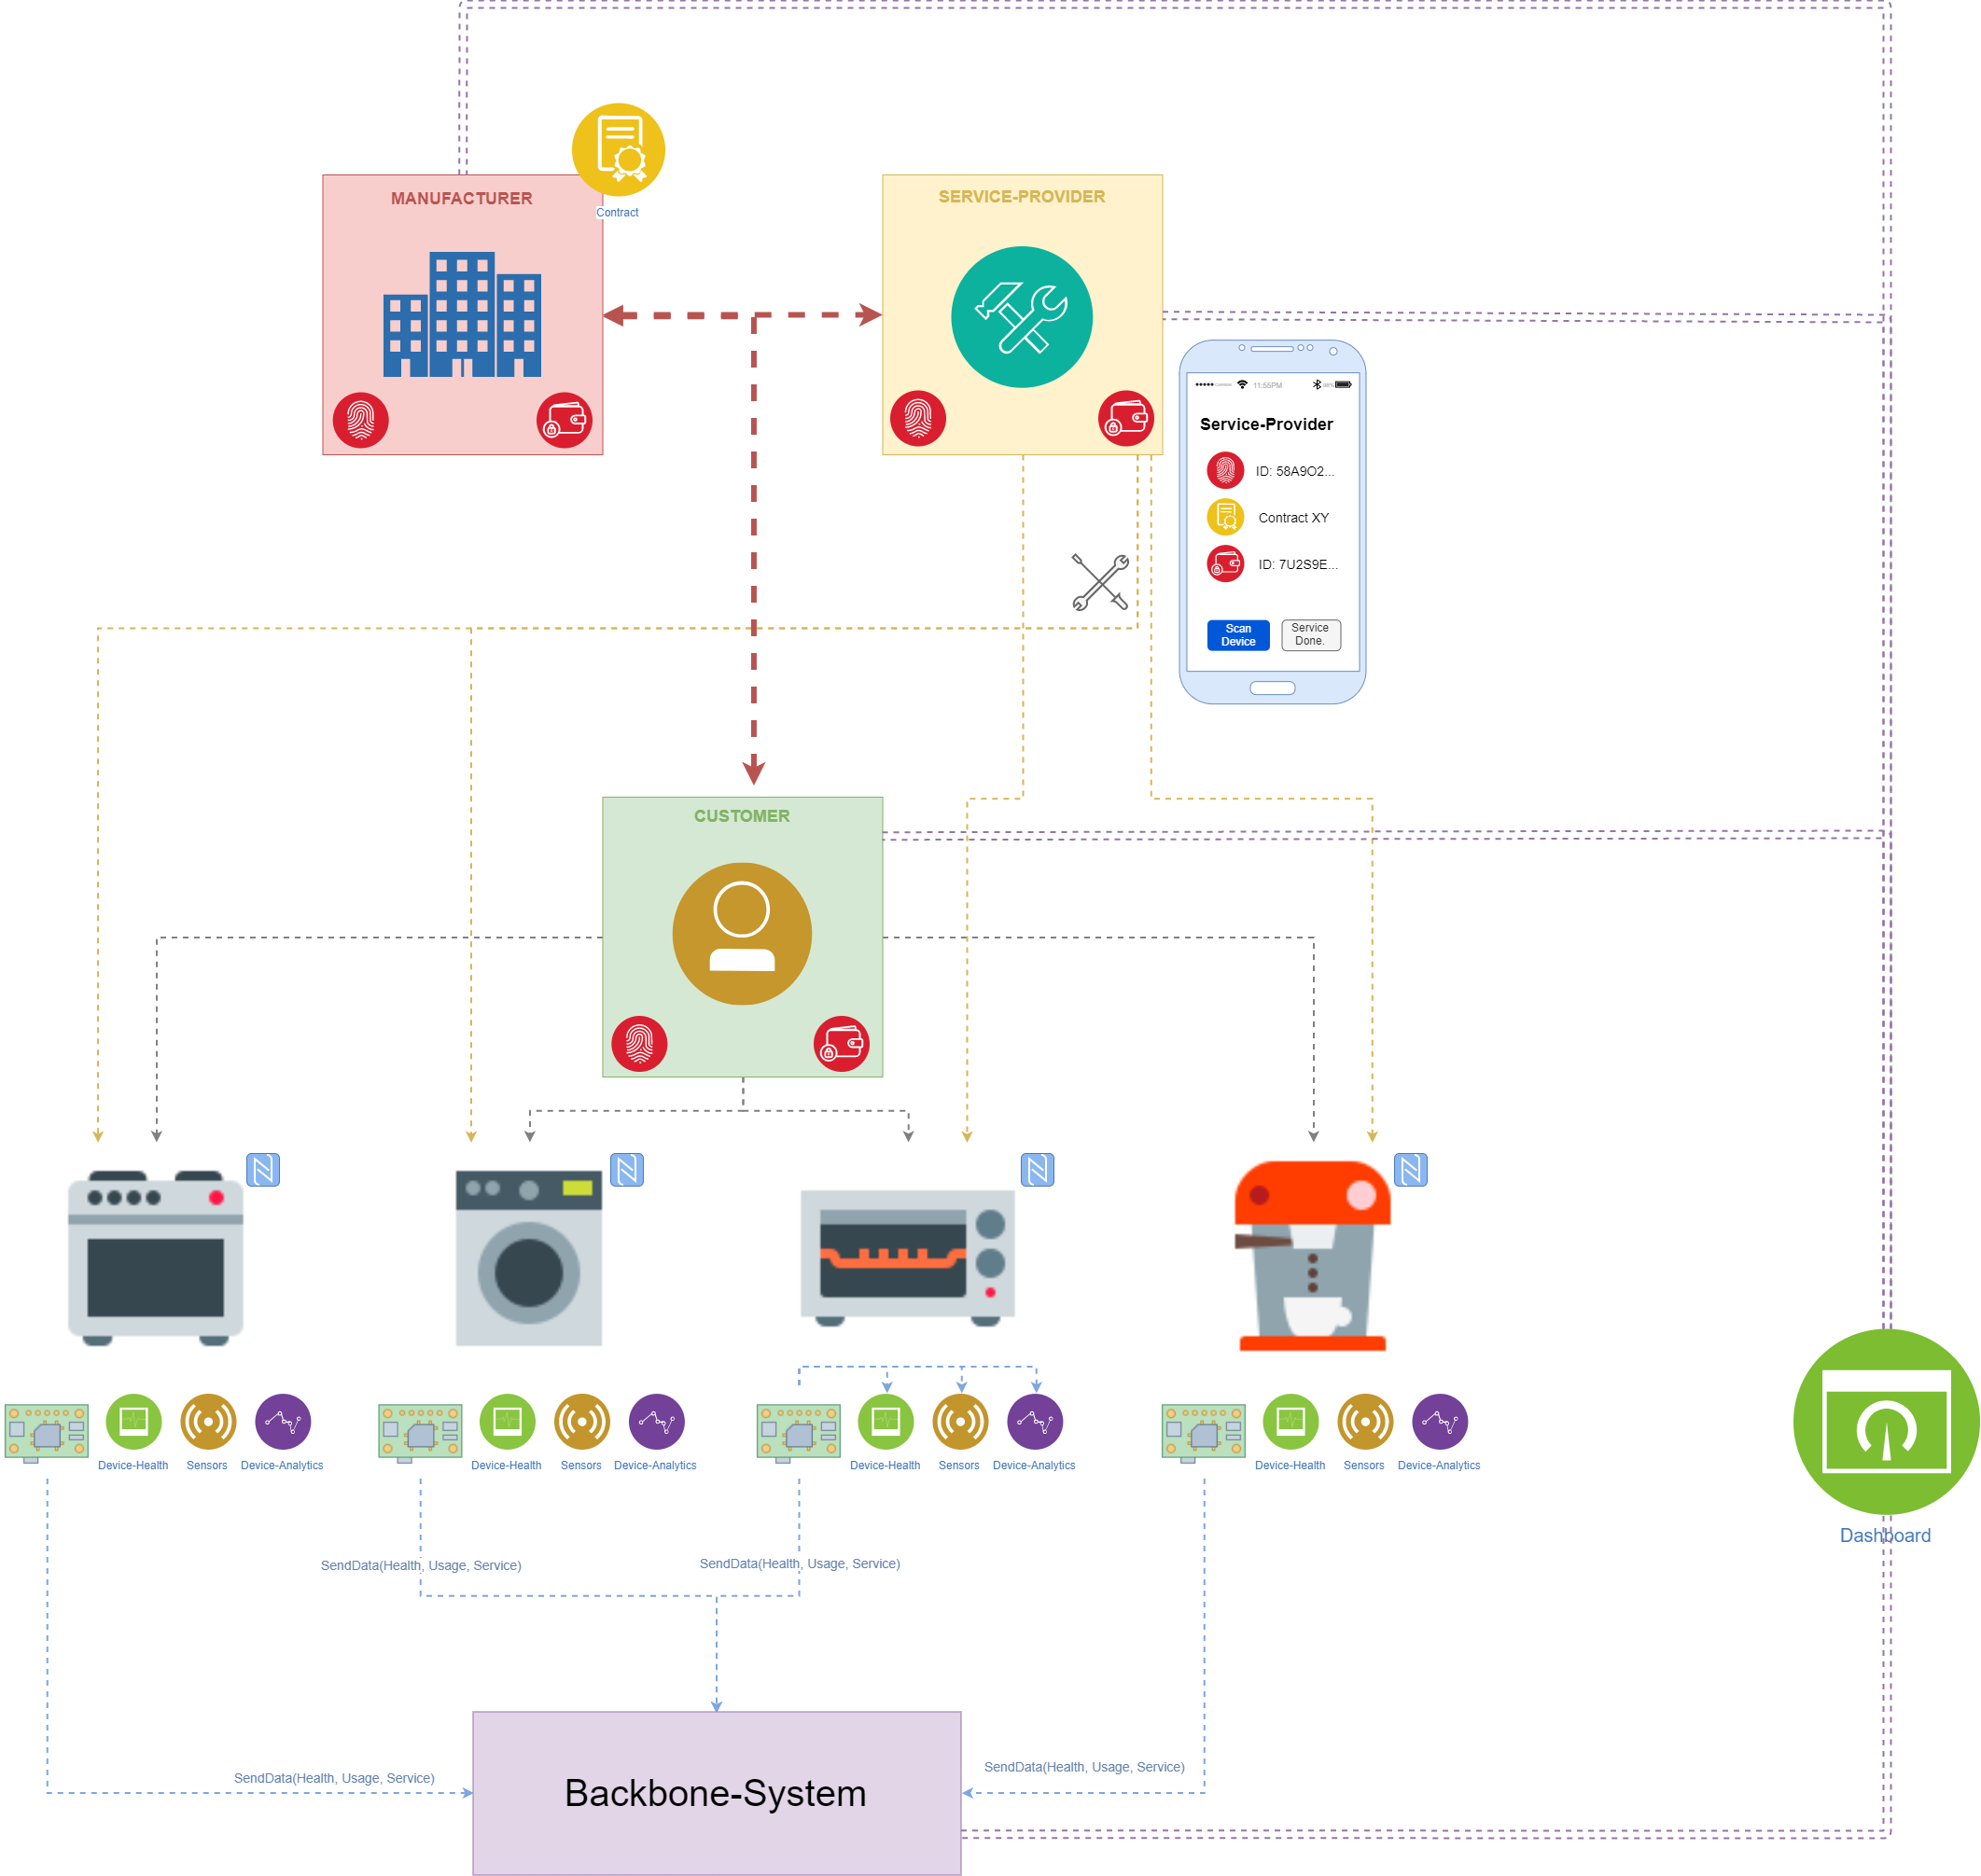
\includegraphics[width=1.0\textwidth]{gfx/IOT-Anwendungsfall.png}
 \caption{Grafische Veranschaulichung des Anwendungsfalls}
 \label{fig:chapter04:usecase}
\end{figure}


Der vorgestellte Anwendungsfall beinhaltet Zusammenspiel mehrerer Stakeholder, welches im Folgenden detailliert beschrieben wird:
\begin{description}
  \item[Hersteller] Der Hersteller der Geräte entwickelt und produziert die zu vermietenden Haushaltsgeräte und bietet diese zur Vermietung an Kunden auf der Plattform an. Er vertreibt Ersatzteile sowie Pflege- und Zusatzprodukte zu seinen Geräten, die Kunden und Service-Dienstleister erwerben können. Der Hersteller kann Service-Dienstleister beauftragen, seine in Vermietung befindlichen Geräte zu warten und zu reparieren. Die dazugehörige Beauftragung und Abrechnung erfolgt über die Plattform. Für vermietete Geräte erhält er nach einem Pay-as-You-Use Prinzip eine Bezahlung der Kunden entsprechend ihres Verbrauches.
  \item[Lieferant] Der Lieferant ist für die Lieferung der Geräte und Zusatzprodukte zu den Kunden und Service-Dienstleistern zuständig. Er holt die Ware beim Hersteller ab und liefert diese an Kunden und Service-Dienstleister; die benötigten Adressinformationen sind auf der Plattform hinterlegt. Die Bezahlung für die Auslieferung erfolgt über die Plattform und berechnet sich automatisch über die Distanz der Lieferstrecke und der Abmessung der Ware.
  \item[Kunde] Der Kunde mietet Geräte vom Hersteller. Die Bestellung und Abrechnung erfolgt über die Plattform nach einem Pay-as-You-Use Prinzip, was bedeutet, dass der Kunde für die tatsächliche Nutzung der Geräte bezahlt und keinen fixen monatlichen Pauschalbetrag. Die Plattform sieht ebenfalls ein Reward-Programm vor, welches dem Kunden für durchgeführte Wartungen und die Pflege der Geräte eine vertraglich festgeschriebene Gutschrift zukommen lässt. Darüber hinaus kann der Kunde auf Wunsch Konsumgüter wie Kaffee und Reinigungsmittel über die Plattform bestellen; dies geschieht vollautomatisch über das Gerät: Sobald die Menge des Produktes ein gewisses Limit unterschreitet, beauftragt das Gerät selbstständig den Kauf und die Anlieferung der Produkte über die Plattform.
  \item[Service-Dienstleister] Der Service-Dienstleister ist zuständig für die Wartung und Reparatur der Geräte und wird über die Plattform beauftragt. Dies kann entweder manuell geschehen, indem der Hersteller den Service-Dienstleister explizit beauftragt, oder voll-automatisch, indem das Gerät selbst den Service-Dienstleister über die Plattform benachrichtigt.
\end{description}

Die Abbildung \ref{fig:chapter04:usecase_workflow} zeigt den groben Ablauf beginnend mit der Mietanfrage eines Kunden bis zur monatlichen Bezahlung der Teilnehmer für ihren Service.

\begin{figure}[htbp]
 \centering
 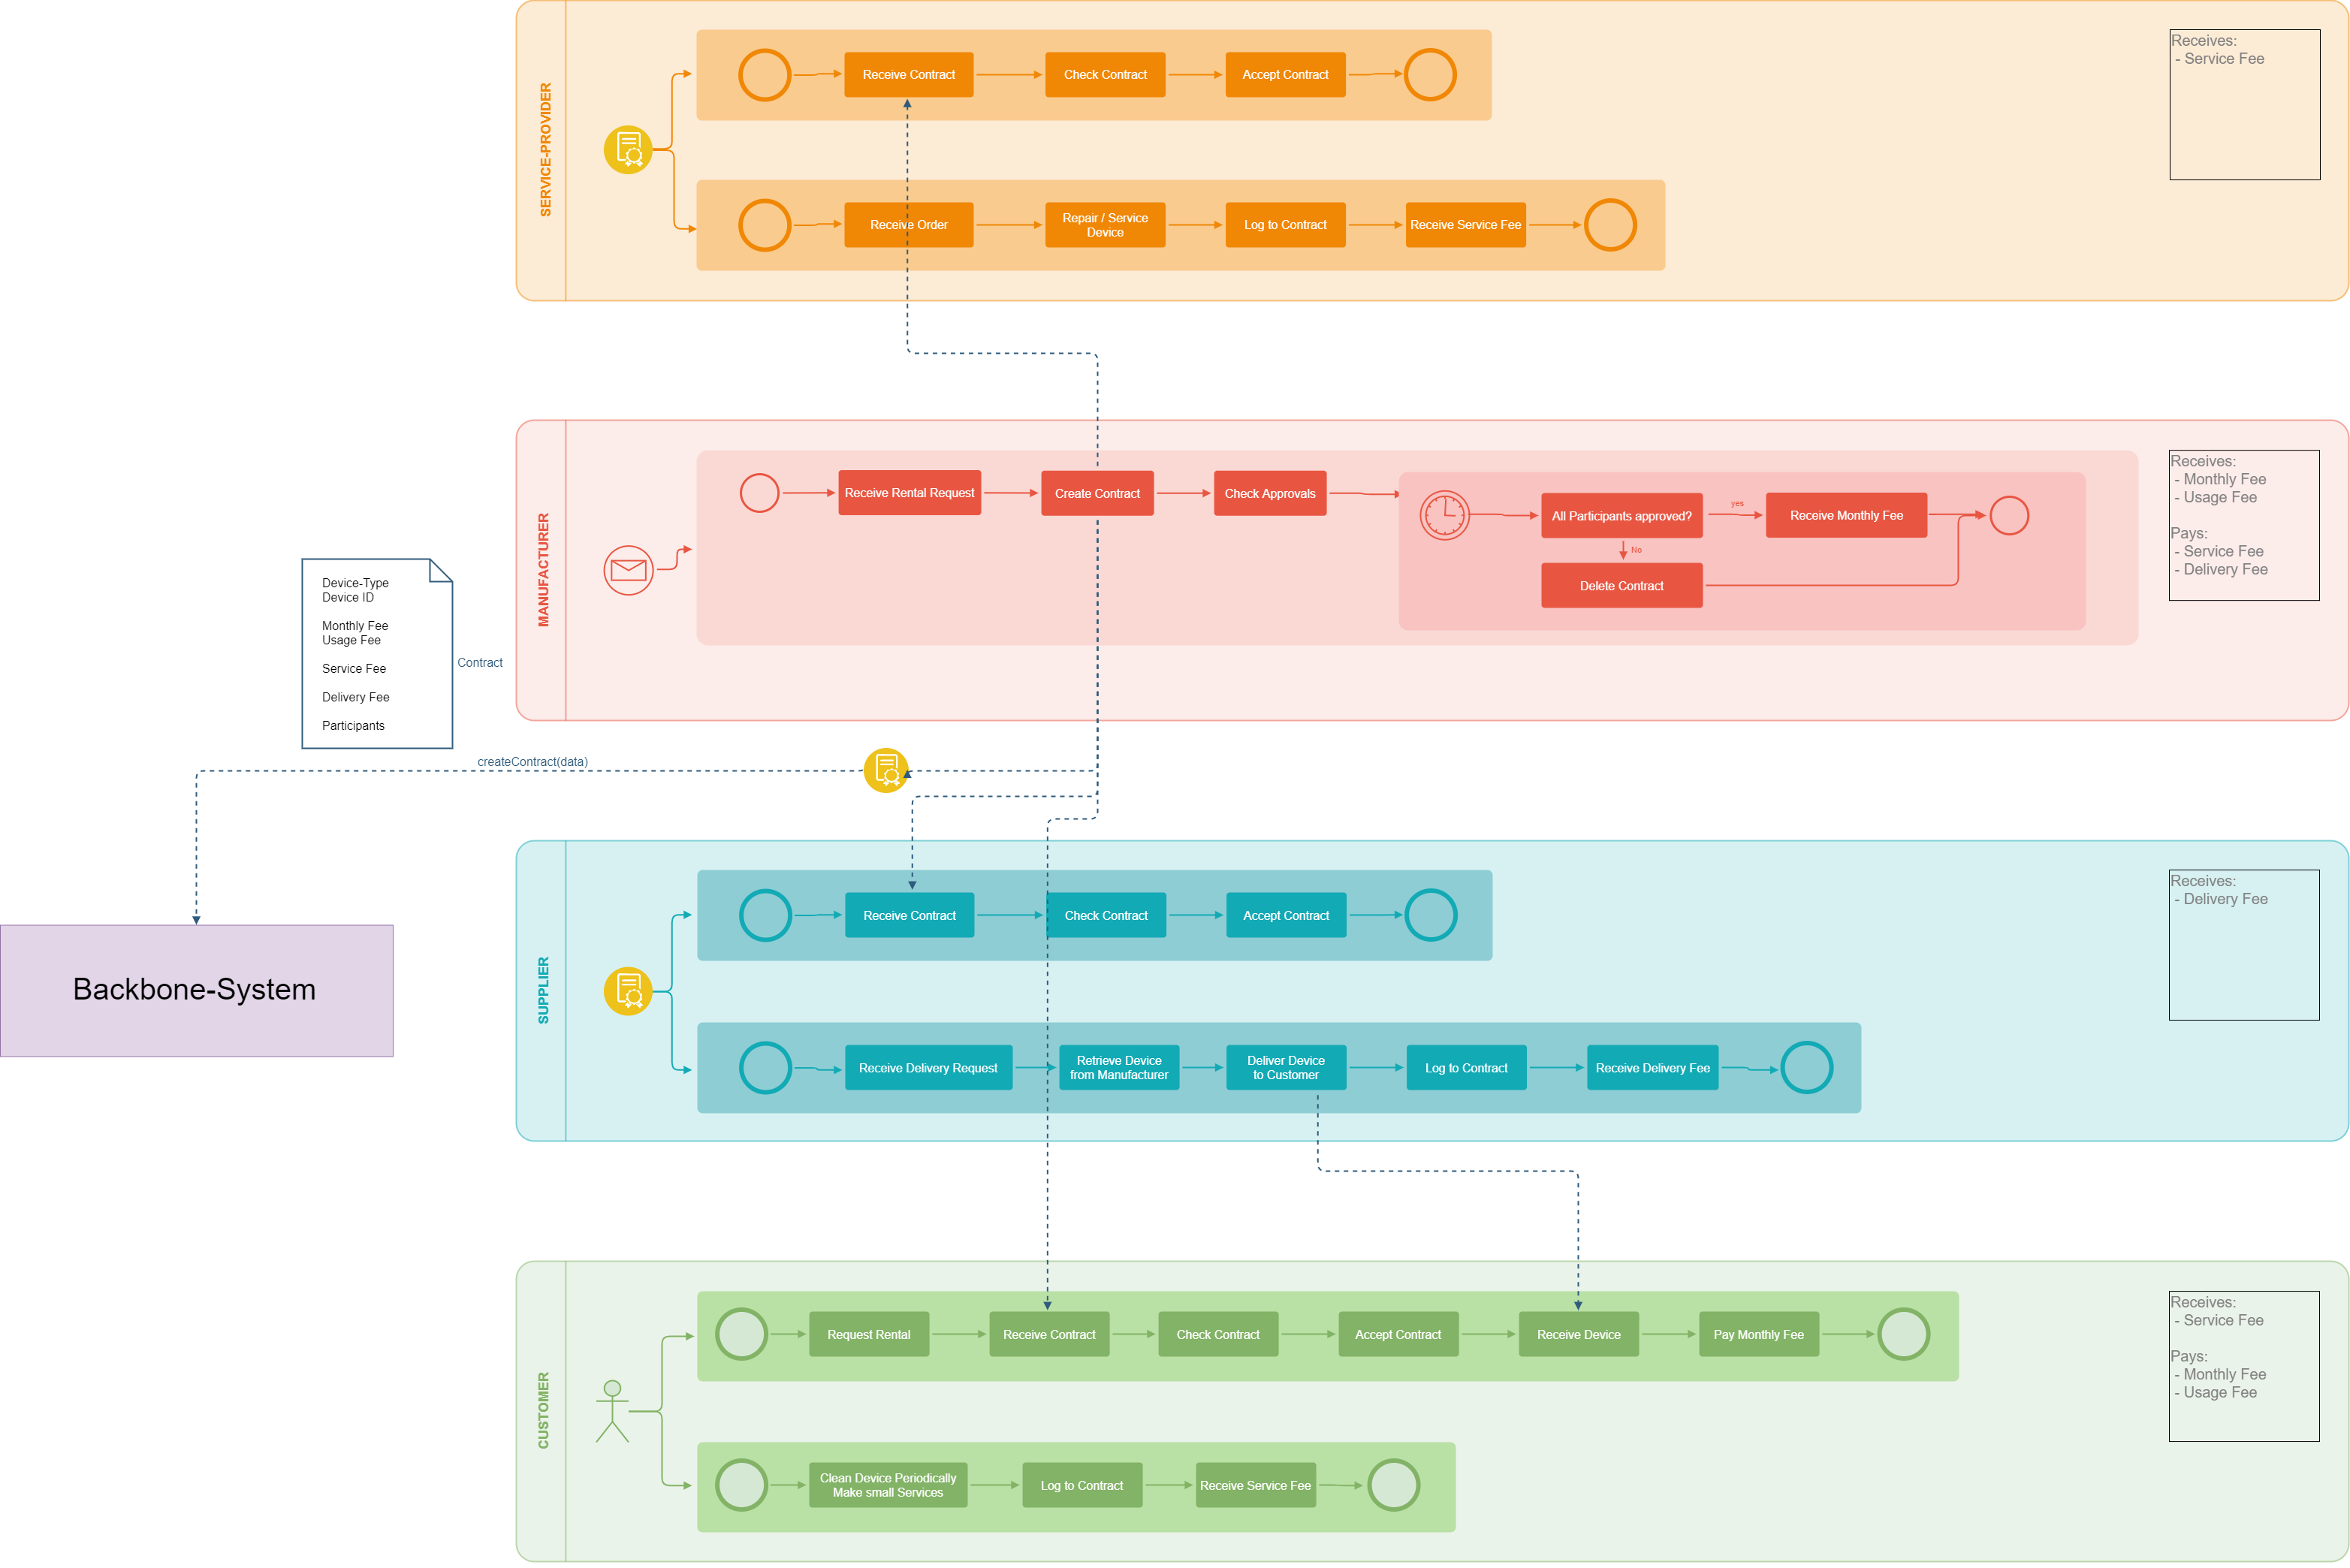
\includegraphics[width=1.0\textwidth]{gfx/IOT-Anwendungsfall_Ablauf.png}
 \caption{Grober Ablauf des Anwendungsfalls}
 \label{fig:chapter04:usecase_workflow}
\end{figure}

%
% Section: Technische Lösungsskizze
%
\section{Technische Lösungsskizze}
\label{sec:iot_usecase:solution}
Diese Arbeit setzt den oben beschriebenen Anwendungsfall prototypisch um. Die Lösungsskizze zeigt, wie der Anwendungsfall in dieser Arbeit technische umgesetzt wird. Der Lösungsansatz bezieht sich dabei auf eine Implementierung auf Basis einer \ac{DLT}. Neben den beteiligten Stakeholdern besteht das Gesamtsystem auf einem Frontend, dass jedem Stakeholder die für ihn relevanten Funktionen zur Verfügung stellt. Das Backend des Systems besteht aus einer \ac{DLT}-Lösung\footnote{Die konkrete Implementierung, die als Backbone-System eingesetzt wird, wird im Laufe dieser Arbeit ermittelt.}.

\subsection{Endgeräte}
\label{subsec:iot_usecase:solution:device}
Jedes Gerät besitzt eine eindeutige Identifikationsnummer und eine eindeutige Referenz zu dessen Eigentümer (Hersteller). Befindet sich ein Gerät in Vermietung, so existiert zwischen dem Mieter (Kunde) und dem Vermieter (Hersteller) ein Vertrag, der auf der zentralen Plattform persistiert wird. Das Gerät hat über das Internet Zugriff auf diese Plattform und damit auf den Vertrag, in dem wichtige Informationen zu den Rahmenbedingungen wie der Dauer des Vertragsverhältnisses sowie die Kostenaufschlüsselung für alle verschiedenen Abrechnungen. Die Sensoren zum Registrieren des Verbrauchs und des Gerätestatus befinden sich auf dem Gerät selbst. Diese melden alle gesammelten Daten an eine Sammelstelle am Gerät. Dort werden die Daten aufbereitet, gemäß Vertrag verarbeitet und gesammelt. In einem vertraglich festgelegten Intervall meldet das Gerät alle relevanten Daten wie Nutzung, Reinigungs- und Wartungsarbeiten und sonstige Informationen an das Backend und den verknüpften Vertrag, der wiederum die entsprechenden Geld-Transfers in die Wege leitet (siehe unten). In Abbildung \ref{fig:chapter04:usecase_device} wird ein Endgerät schematisch dargestellt.

\begin{figure}[htbp]
 \centering
 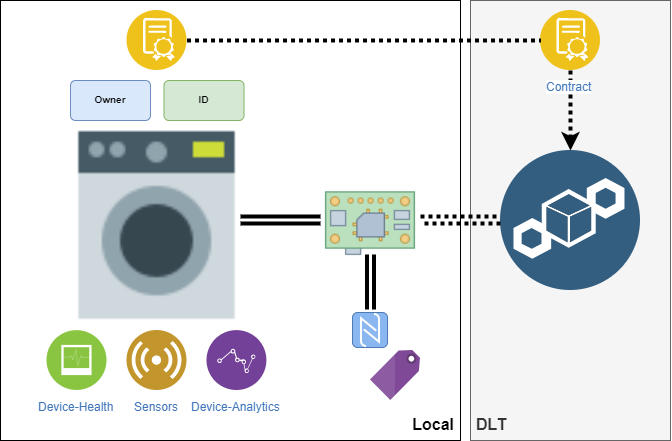
\includegraphics[width=1.0\textwidth]{gfx/IOT-Anwendungsfall_Device.png}
 \caption{Aufbau und Bestandteile eines Endgeräts}
 \label{fig:chapter04:usecase_device}
\end{figure}

\subsection{Verträge}
\label{subsec:iot_usecase:solution:contracts}
Mietverträge werden von allen beteiligten Parteien digital unterschrieben und im Backend gespeichert. Sie halten verschiedene Informationen, unter Anderem über die Vertragslaufzeit, die Kosten sowie die zu erbringenden Leistungen der Parteien. Der Vertrag beinhaltet Mechanismen zur Begutschriftung und zur Belastung der Konten aller Beteiligten; die folgende Auflistung nennt alle wichtigen Geld-Transfers:
\begin{itemize}
  \item Nutzung durch den Kunden (Sender ist der Kunde, Empfänger ist der Hersteller)
  \item Reinigung durch den Kunden / Service-Dienstleister (Sender ist der Hersteller, Empfänger ist der Kunde / der Service-Dienstleister)
  \item Wartung durch den Kunden / Service-Dienstleister (Sender ist der Hersteller, Empfänger ist der Kunde / der Service-Dienstleister)
  \item Lieferung durch den Lieferanten (Sender ist der Absender, Empfänger ist die Lieferant)
\end{itemize}

\subsection{Frontend}
\label{subsec:iot_usecase:solution:frontend}
Das Frontend stellt eine grafische Benutzerschnittstelle bereit, die je nach Stakeholder die relevanten Informationen und Funktionalitäten bereitstellt:
\begin{description}
  \item[Hersteller-Ansicht] Eine Übersicht über alle Geräte sowie deren Status, ob sie sich derzeit in Vermietung befinden, gibt dem Hersteller Aufschluss über die momentane Gesamtlage. Laufende Verträge können eingesehen und aktuelle Mietanfragen bearbeitet werden.
  \item[Kunden-Ansicht] Als Kunde kann ich nach erfolgreicher Authentifizierung meine gemieteten Geräte sowie die damit verbundenen, laufenden Verträge einsehen. Ich habe Zugang zu den Verbrauchs- und Statusinformationen, die meine Geräte an die Plattform übermitteln und habe somit vollkommene Transpranz über meine laufenden Kosten. Laufende Verträge kann ich vertragsgerecht kündigen und bearbeiten sowie neue Verträge abschließen. Neue Mietanträge, die ich an den Hersteller gestellt habe, kann ich verfolgen und entsprechende Informationen über den Lieferstatus abfragen. Zusatzkonfigurationen wie zum Beispiel meine bedarfs- und verbrauchsabhängige Kaffeelieferung für die gemietete Kaffeemaschine kann ich ebenfalls beauftragen.
  \item[Service-Dienstleister-Ansicht] Nach erfolgreicher Authentifizierung als Service-Dienstleister habe ich Einsicht auf alle aktuell laufenden Service-Verträge. Ich sehe alle Meldungen über Service-Anfragen und Aufträge, die in nächster Zeit anstehen. Eine Auflistung der Einnahmen durch Reparaturen und Services sowie meinen Kontostand kann ich ebenfalls einsehen.
  \item[Lieferanten-Ansicht] Nach erfolgreicher Authentifizierung als Service-Dienstleister habe ich Einsicht auf alle aktuell laufenden Liefer-Verträge. Ich sehe alle Meldungen über Liefer-Anfragen, die in nächster Zeit anstehen. Eine Auflistung der Einnahmen durch Lieferungen sowie meinen Kontostand kann ich ebenfalls einsehen.
\end{description}

\subsection{Backend}
\label{subsec:iot_usecase:solution:backend}
Das Backend wird in dieser praktischen Verprobung mittels eines \ac{DLT} realisiert. Als dezentrale Plattform verwaltet und speichert es alle Verträge (in diesem Kontext: Smart-Contracts) sowie die Identitäten und Konten (Wallets) der oben aufgelisteten Stakeholder.
